%%%%%%%%%%%%%%%%%%%%%%%%%%%%%%%%%%%%%%%%%%%%%%%%%%%
%% P3: Phenomenology of Particle Physics                         
%%
%% Author:  André Rubbia                   		 
%%
%% Figure 1.2 Illustration of the strength of the fundamental forces as a function of the energy scale.
%%
%% This work is licensed under the Creative Commons Attribution 4.0 International License. 
%% To view a copy of this license, visit http://creativecommons.org/licenses/by/4.0/ or 
%% send a letter to Creative Commons, PO Box 1866, Mountain View, CA 94042, USA.
%%
%%%%%%%%%%%%%%%%%%%%%%%%%%%%%%%%%%%%%%%%%%%%%%%%%%%

\documentclass[a4paper,10pt]{article}

\usepackage[T1]{fontenc}
\usepackage[utf8]{inputenc}
\usepackage{lmodern}
\usepackage[labelfont=bf]{caption}

\usepackage{tikz}
\usepackage{pgfplots}
\pgfplotsset{compat=1.17}
\usepgfplotslibrary{ternary}
\usepgfplotslibrary{fillbetween}
\usepgfplotslibrary{external}

\def\d{\mathrm{d}}

\begin{document}

%%%%%%%%%%%%%%%   FIGURE  %%%%%%%%%%%%%%%%%%%%%%%%%%%%%%
\begin{figure}[htb]
    \centering
    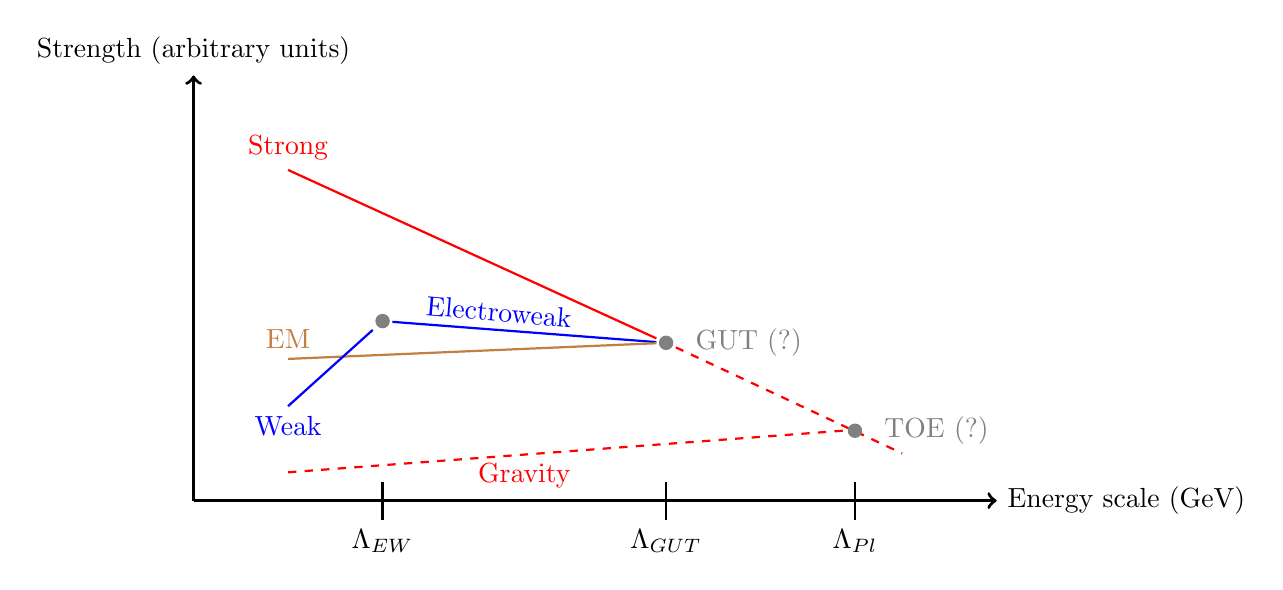
\begin{tikzpicture}[scale=1.2]
        \draw[very thick,->] (0,0) -- (8.5,0) node[right] {Energy scale (GeV)};
        \draw[very thick,->] (0,0) -- (0,4.5) node[above] {Strength (arbitrary units)};
        \draw[thick] (2,0.2) -- (2,-0.2) node[below] {$\Lambda_{EW}$};
        \draw[thick] (5,0.2) -- (5,-0.2) node[below] {$\Lambda_{GUT}$};
        \draw[thick] (7,0.2) -- (7,-0.2) node[below] {$\Lambda_{Pl}$};
        \node (GUT) at (5,1.67) {};
        \node (EW) at (2,1.9) {};
        \draw[dashed,thick,red] (GUT) --  (7.5,0.5);
        \node[above,red] at (1,3.5) {Strong} ;
        \draw[thick,red] (1,3.5) --  (GUT);
        \draw[dashed,thick,red] (1,0.3) --  (7,0.75);
        \draw[thick,blue] (EW) --  (GUT);
        \draw[thick,brown] (1,1.5) node[above] {EM} --  (GUT)  ;
        \draw[thick,blue] (1,1) node[below] {Weak} --  (EW) ;
        \node[blue,below,rotate=-5] at (3.25,2.2) {Electroweak};
        \node[red,below] at (3.5,0.5) {Gravity};
        \filldraw [gray] (EW) circle (2pt);
        \filldraw [gray] (GUT) circle (2pt) node[right=0.25cm] {GUT (?)};
        \filldraw [gray] (7,0.74) circle (2pt) node[right=0.25cm] {TOE (?)};
    \end{tikzpicture}
    \caption{Illustration of the strength of the fundamental forces as a function of the energy scale.
    At the highest energies all forces should unify.}
\end{figure}%
%
%%%%%%%%%%%%%%%   END FIGURE  %%%%%%%%%%%%%%%%%%%%%%%%%%%%%%
%

\end{document}
